\documentclass[12pt,a4paper]{article}
\usepackage[utf8]{inputenc}
\usepackage[margin=3cm]{geometry} % margins
%\linespread{1.2} % line spacing
\usepackage{graphicx} % Required for inserting images
\usepackage{hyperref}
\usepackage{subcaption}
\usepackage{float}
\usepackage{tcolorbox}
\usepackage{amsmath}
\usepackage{amssymb}
\usepackage{listings}% http://ctan.org/pkg/listings}
\usepackage{algorithm}
\usepackage{algorithmic}
\usepackage[toc,page]{appendix}
\usepackage{multicol}
\usepackage{siunitx}
\usepackage{comment}
\usepackage{xcolor}
\usepackage{caption}
\usepackage{forest}
\usepackage{tikz}
\usetikzlibrary{shapes.geometric, arrows}
\usepackage{todonotes} %\setuptodonotes{tickmarkheight=4pt}

\newtheorem{definition}{Definition}

\tikzstyle{startstop} = [rectangle, rounded corners, 
minimum width=3cm, 
minimum height=1cm,
text centered, 
draw=black, 
fill=red!30]

\tikzstyle{io} = [trapezium, 
trapezium stretches=true, % A later addition
trapezium left angle=70, 
trapezium right angle=110, 
minimum width=3cm, 
minimum height=1cm, text centered, 
draw=black, fill=blue!30]

\tikzstyle{process} = [rectangle, 
minimum width=3cm, 
minimum height=1cm, 
text centered, 
text width=3cm, 
draw=black, 
fill=orange!30]

\tikzstyle{decision} = [diamond, 
minimum width=3cm, 
minimum height=1cm, 
text centered, 
draw=black, 
fill=green!30]
\tikzstyle{arrow} = [thick,->,>=stealth]

% To delete lstlisting caption "Listing x"
%\captionsetup[lstlisting]{labelformat=empty}

\lstdefinestyle{myStyle}{
    belowcaptionskip=1\baselineskip,
    breaklines=true,
    frame=none,
    numbers=none, 
    basicstyle=\footnotesize\ttfamily,
    keywordstyle=\bfseries\color{green!40!black},
    commentstyle=\itshape\color{purple!40!black},
    identifierstyle=\color{black},
    backgroundcolor=\color{white},
}

\lstdefinestyle{csvStyle}{
    basicstyle=\ttfamily\small, % Use a typewriter font
    columns=fullflexible, % Better column alignment
    %frame=single, % Add a border
    %backgroundcolor=\color{gray!10}, % Light gray background
    keywordstyle=\color{blue}\bfseries, % Style for keywords (optional)
    morekeywords={name,code,loc_latitude,loc_longitude, ATM_id, city, country,
    number_id, client_id, expiration, CVC, extract_limit, amount_avg_withdrawal,amount_std_withdrawal,withdrawal_day,
    amount_avg_deposit,amount_std_deposit,deposit_day,inquiry_day,
    amount_avg_transfer,amount_std_transfer,transfer_day,
    transaction_id,number_id,ATM_id,transaction_type,transaction_start,
    transaction_end, transaction_amount}, % Highlight CSV headers as keywords
    showstringspaces=false,
    captionpos=b,                    % sets the caption-position to bottom
}

\lstdefinestyle{cypherStyle}{
    backgroundcolor=\color{white},   % choose the background color
    basicstyle=\footnotesize\ttfamily,        % the size of the fonts that are used for the code
    commentstyle=\itshape\color{purple!40!black},
    keywordstyle=\bfseries\color{green!40!black},
    breakatwhitespace=false,         % sets if automatic breaks should only happen at whitespace
    breaklines=true,                 % sets automatic line breaking
    captionpos=b,                    % sets the caption-position to bottom
    commentstyle=\color{gray},    % comment style
    deletekeywords={},            % if you want to delete keywords from the given language
    escapeinside={\%*}{*)},          % if you want to add LaTeX within your code
    extendedchars=true,              % lets you use non-ASCII characters; for 8-bits encodings only, does not work with UTF-8
    %firstnumber=1000,                % start line enumeration with line 1000
    frame=none,                    % adds a frame around the code
    keepspaces=true,                 % keeps spaces in text, useful for keeping indentation of code (possibly needs columns=flexible)
    language=SQL,                    % the language of the code
    morekeywords={*,IF, REQUIRE, FOR, IS, LOAD, CSV, WITH, HEADERS, MERGE, toFloat, toInteger, date},            % if you want to add more keywords to the set
    numbers=none,                    % where to put the line-numbers; possible values are (none, left, right)
    numbersep=5pt,                   % how far the line-numbers are from the code
    numberstyle=\tiny\color{mygray}, % the style that is used for the line-numbers
    rulecolor=\color{black},         % if not set, the frame-color may be changed on line-breaks within not-black text (e.g. comments (green here))
    showspaces=false,                % show spaces everywhere adding particular underscores; it overrides 'showstringspaces'
    showstringspaces=false,          % underline spaces within strings only
    showtabs=false,                  % show tabs within strings adding particular underscores
    stepnumber=1,                    % the step between two line-numbers. If it's 1, each line will be numbered
    stringstyle=\ttfamily,     % string literal style
    tabsize=2,                       % sets default tabsize to 2 spaces
}

%% Golang definition for listings
%% http://github.io/julienc91/lstlistings-golang
%%
\lstdefinelanguage{Golang}%
  {morekeywords=[1]{package,import,func,type,struct,return,defer,panic,%
     recover,select,var,const,iota,},%
   morekeywords=[2]{string,uint,uint8,uint16,uint32,uint64,int,int8,int16,%
     int32,int64,bool,float32,float64,complex64,complex128,byte,rune,uintptr,%
     error,interface},%
   morekeywords=[3]{map,slice,make,new,nil,len,cap,copy,close,true,false,%
     delete,append,real,imag,complex,chan,},%
   morekeywords=[4]{for,break,continue,range,go,goto,switch,case,fallthrough,if,%
     else,default,},%
   morekeywords=[5]{Println,Printf,Error,Print,},%
   sensitive=true,%
   morecomment=[l]{//},%
   morecomment=[s]{/*}{*/},%
   morestring=[b]',%
   morestring=[b]",%
   morestring=[s]{`}{`},%
}

\lstdefinestyle{golangStyle}{
    captionpos=b,              % sets the caption-position to bottom
    belowcaptionskip=1\baselineskip,
    breaklines=true,
    frame=none,
    numbers=none, 
    basicstyle=\footnotesize\ttfamily,
    keywordstyle=\bfseries\color{green!40!black},
    commentstyle=\scriptsize\itshape\color{gray},
    identifierstyle=\color{black},
    backgroundcolor=\color{white},
    language=Golang,
    tabsize=1,                 % reduces the tab size (number of spaces per tab)
    keepspaces=true,           % preserves spaces and tabs exactly as written
    showspaces=false,          % hides visible spaces
    showtabs=false             % hides visible tabs
}

\setlength{\parindent}{0pt} % QUITAR SANGRÍAS
\captionsetup{font=small} % Fuente del texto de las imagenes

\newcommand{\DP}{$\mathsf{DP}$ }
\newcommand{\DPATM}{$\mathsf{DP_{ATM}}$ }

\newcommand{\alertch}{$\mathsf{alert}$ }
\newcommand{\eventch}{$\mathsf{event}$ }
\newcommand{\internaledgech}{$\mathsf{internal\_edge}$ }

\newcommand{\cardsubgraph}{$\mathsf{cs}$ }

\newcommand{\filter}{\emph{Filter} }
\newcommand{\source}{\emph{Source} }
\newcommand{\sink}{\emph{Sink} }
\newcommand{\generator}{\emph{Generator} }
\newcommand{\filterworker}{\emph{Filter Worker} }

\newcommand{\F}{$\mathsf{F}$ }
\newcommand{\Sr}{$\mathsf{Sr}$ }
\newcommand{\Sk}{$\mathsf{Sk}$ }
\newcommand{\G}{$\mathsf{G}$ }
\newcommand{\FW}{$\mathsf{FW}$ }
\newcommand{\smallG}{$\mathsf{GDB_A}$}
\newcommand{\mediumG}{$\mathsf{GDB_B}$}

\newenvironment{graysection}
  {\begingroup\color{gray}} % Start with gray color
  {\endgroup}               % End the color group

%%%%%%%
\newcommand{\ep}[1]{\todo[inline,backgroundcolor=orange!70,textcolor=black]{\tiny \textbf{Edelmira:} #1}}
%%%%%%
%%%%%%%
\newcommand{\fmc}[1]{\todo[inline,backgroundcolor=blue!40,textcolor=black]{\small \textbf{Fernando:} #1}}
%%%%%%

%%%%%%%
\newcommand{\ad}[1]{\todo[inline,backgroundcolor=green!40,textcolor=black]{\tiny \textbf{Amalia:} #1}}
%%%%%%

\title{TFM-FernandoMartín}
\author{Fernando Martín Canfrán}
\date{\today}

\begin{document}

\maketitle


\newpage
\newpage
\section{Analysis of results}


\begin{figure}[H]
    \centering
    % Temporarily adjust margins for wider content
    \hspace*{-3cm} % Move content to the left by 2 cm (adjust as needed)
    \begin{minipage}{0.5\textwidth}
        \centering
        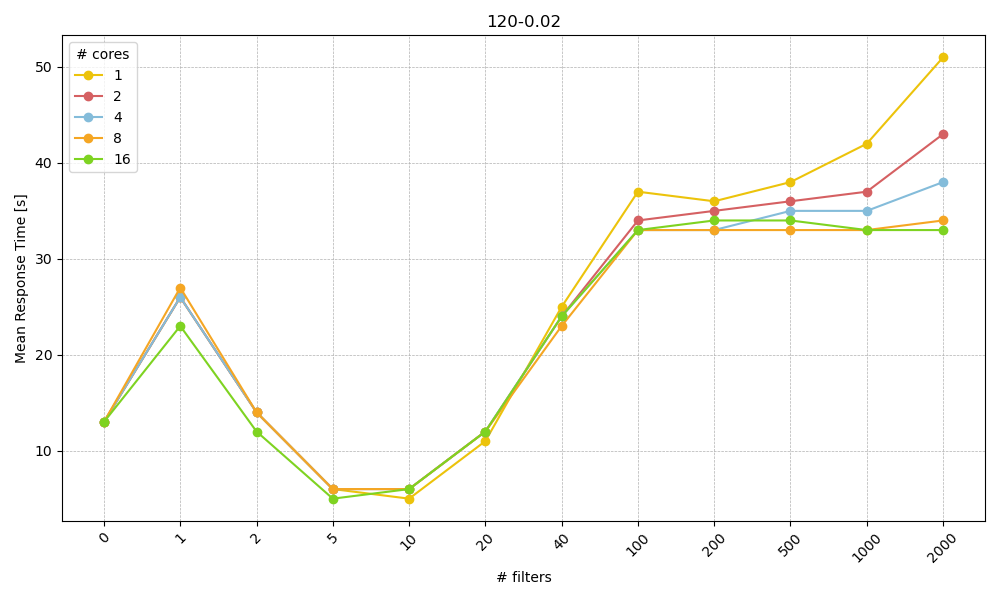
\includegraphics[scale=0.4]{images/4-Experiments/NRT/small/120-0.02/combined/plots/mrt-1.png}
        \caption*{}
    \end{minipage}
    \hspace{0.16\textwidth}
    \begin{minipage}{0.5\textwidth}
        \centering
        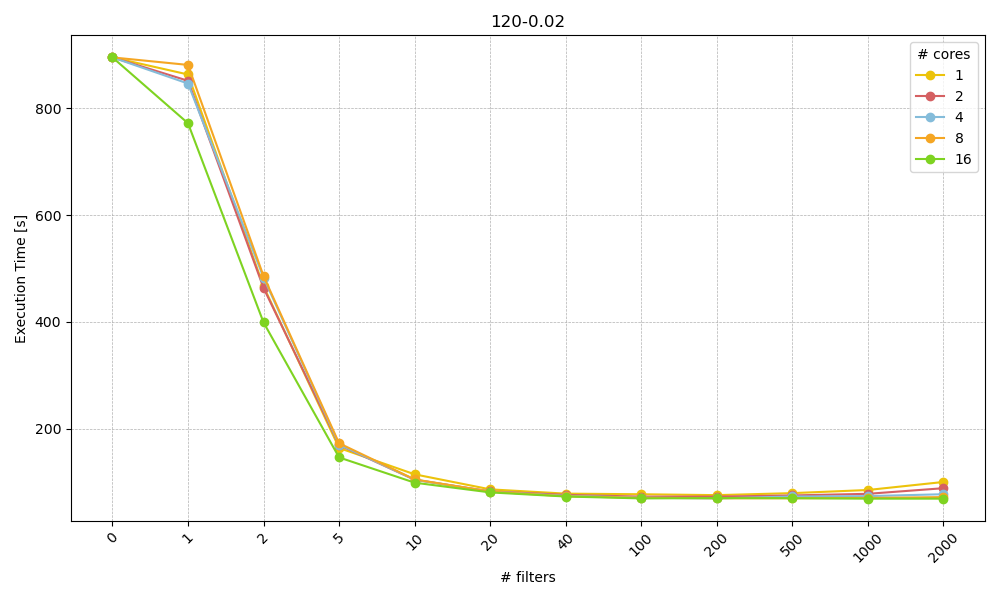
\includegraphics[scale=0.4]{images/4-Experiments/NRT/small/120-0.02/combined/plots/execTime-1.png}
        \caption*{}
    \end{minipage}
    
    \vspace{0.5cm} % Vertical space between rows

    \hspace*{-3cm} % Move content to the left for the second row
    \begin{minipage}{0.5\textwidth}
        \centering
        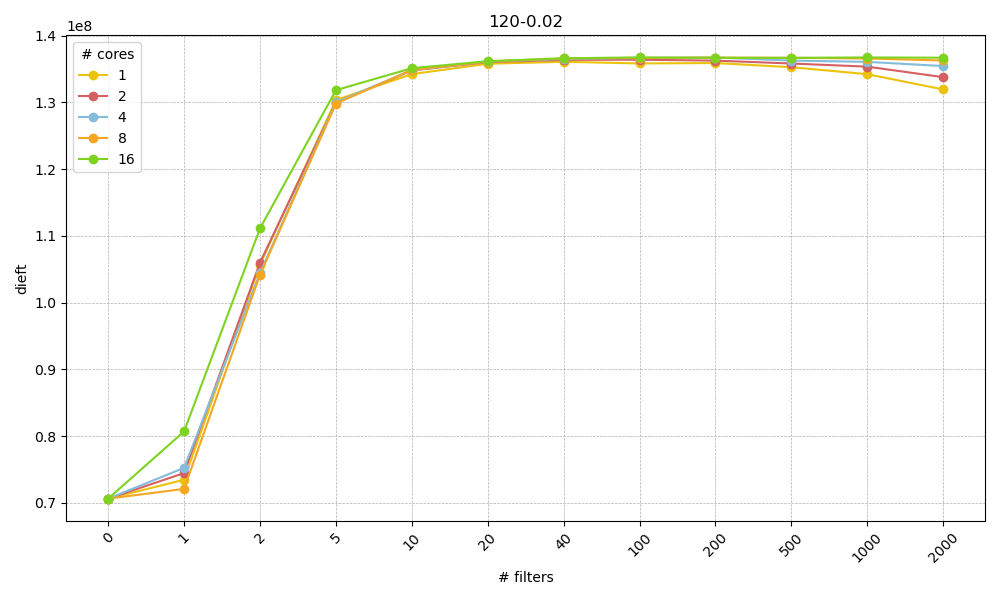
\includegraphics[scale=0.4]{images/4-Experiments/NRT/small/120-0.02/combined/plots/dieft-1.png}
        \caption*{}
    \end{minipage}
    \hspace{0.16\textwidth}
    \begin{minipage}{0.5\textwidth}
        \centering
        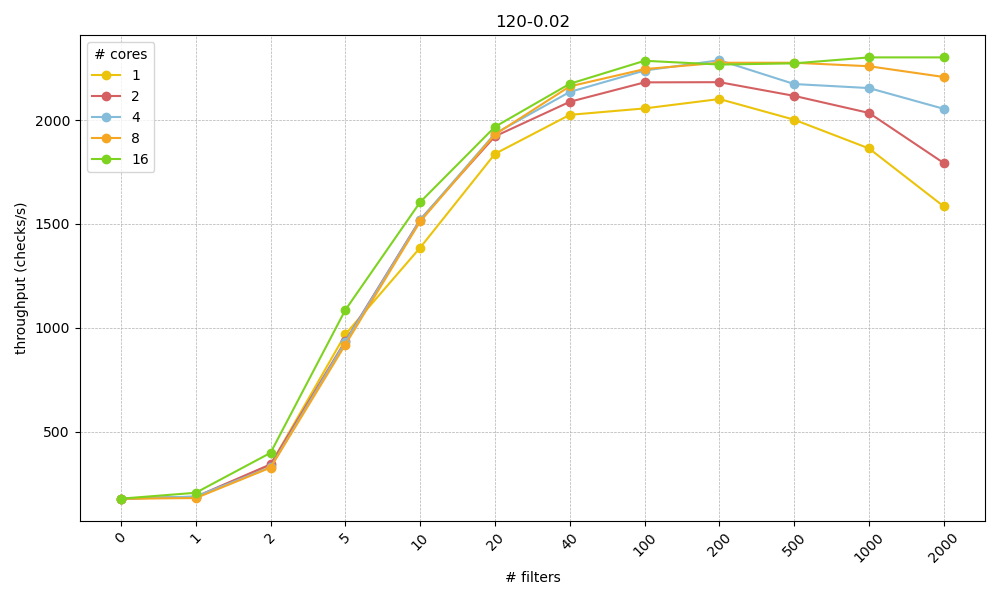
\includegraphics[scale=0.4]{images/4-Experiments/NRT/small/120-0.02/combined/plots/throughput-1.png}
        \caption*{}
    \end{minipage}

    \caption{Combined cores and filters variation plots for big stream: 120-0.02}
    \label{img:exps-small-120-combined}
\end{figure}


















































\newpage
\begin{figure}[H]
    \centering
    % Temporarily adjust margins for wider content
    \makebox[\textwidth][c]{%
        \begin{minipage}{0.5\textwidth}
            \centering
            \includegraphics[scale=0.5]{images/4-Experiments/NRT/small/30-0.02/fixedcores-seq/16c/plots/execTime.png}
            \caption*{30-0.02}
        \end{minipage}
        \hspace{0.1\textwidth}
        \begin{minipage}{0.5\textwidth}
            \centering
            \includegraphics[scale=0.5]{images/4-Experiments/NRT/small/60-0.02/fixedcores-seq/16c/execTime.png}
            \caption*{60-0.02}
        \end{minipage}
    }
    
    \vspace{0.5cm} % Vertical space between rows

    \makebox[\textwidth][c]{%
        \begin{minipage}{0.5\textwidth}
            \centering
            \includegraphics[scale=0.5]{images/4-Experiments/NRT/small/120-0.02/16c/execTime.png}
            \caption*{120-0.02}
        \end{minipage}
    }

    \caption{Execution Time Plots for 16c}
    \label{img:exps-small-execTime-16c}
\end{figure}

\newpage
\paragraph{MRT plots - for a core number 16 - different stream sizes\\}
\newpage

\begin{figure}[H]
    \centering
    % Temporarily adjust margins for wider content
    \makebox[\textwidth][c]{%
        \begin{minipage}{0.5\textwidth}
            \centering
            \includegraphics[scale=0.5]{images/4-Experiments/E1-NRT/30-0.02/16c/mrt.png}
            \caption*{30-0.02}
        \end{minipage}
        \hspace{0.1\textwidth}
        \begin{minipage}{0.5\textwidth}
            \centering
            \includegraphics[scale=0.5]{images/4-Experiments/E1-NRT/60-0.02/16c/mrt.png}
            \caption*{60-0.02}
        \end{minipage}
    }
    
    \vspace{0.5cm} % Vertical space between rows

    \makebox[\textwidth][c]{%
        \begin{minipage}{0.5\textwidth}
            \centering
            \includegraphics[scale=0.5]{images/4-Experiments/E1-NRT/120-0.02/16c/mrt.png}
            \caption*{120-0.02}
        \end{minipage}
    }

    \caption{MRT Plots for 16c}
    \label{img:exps-small-mrt-16c}
\end{figure}

\paragraph{Trace and response time trace for 16c and big stream\\}
\newpage

\begin{figure}[H]
    \centering
    % Subfigures arranged vertically
    \begin{subfigure}[b]{\textwidth}
        \centering
        \includegraphics[scale=0.5]{images/4-Experiments/E1-NRT/30-0.02/16c/traces-response-time-reduced.png}
        \caption{30-0.02}
    \end{subfigure}
    
    \vspace{0.5cm} % Vertical space between subfigures
    \begin{subfigure}[b]{\textwidth}
        \centering
        \includegraphics[scale=0.5]{images/4-Experiments/E1-NRT/60-0.02/16c/traces-response-time-reduced.png}
        \caption{60-0.02}
    \end{subfigure}
    
    \vspace{0.5cm} % Vertical space between subfigures
    \begin{subfigure}[b]{\textwidth}
        \centering
        \includegraphics[scale=0.5]{images/4-Experiments/E1-NRT/120-0.02/16c/traces-response-time-reduced.png}
        \caption{120-0.02}
    \end{subfigure}

    \caption{Response Time Traces for 16c}
    \label{img:exps-small-responsetimetraces-16c}
\end{figure}

\paragraph{Trace and response time trace for 16c and big stream\\}

\begin{figure}[H]
    \centering
    % Subfigures arranged vertically
    \begin{subfigure}[b]{\textwidth}
        \centering
        \includegraphics[scale=0.5]{images/4-Experiments/E1-NRT/30-0.02/16c/traces.png}
        \caption{30-0.02}
    \end{subfigure}
    
    \vspace{0.5cm} % Vertical space between subfigures
    \begin{subfigure}[b]{\textwidth}
        \centering
        \includegraphics[scale=0.5]{images/4-Experiments/E1-NRT/60-0.02/16c/traces.png}
        \caption{60-0.02}
    \end{subfigure}
    
    \vspace{0.5cm} % Vertical space between subfigures
    \begin{subfigure}[b]{\textwidth}
        \centering
        \includegraphics[scale=0.5]{images/4-Experiments/E1-NRT/120-0.02/16c/traces.png}
        \caption{120-0.02}
    \end{subfigure}

    \caption{Results Traces for 16c}
    \label{img:exps-small-traces-16c}
\end{figure}

\begin{figure}[H]
    \centering
    % Temporarily adjust margins for wider content
    \hspace*{-3cm} % Move content to the left by 2 cm (adjust as needed)
    \begin{minipage}{0.5\textwidth}
        \centering
        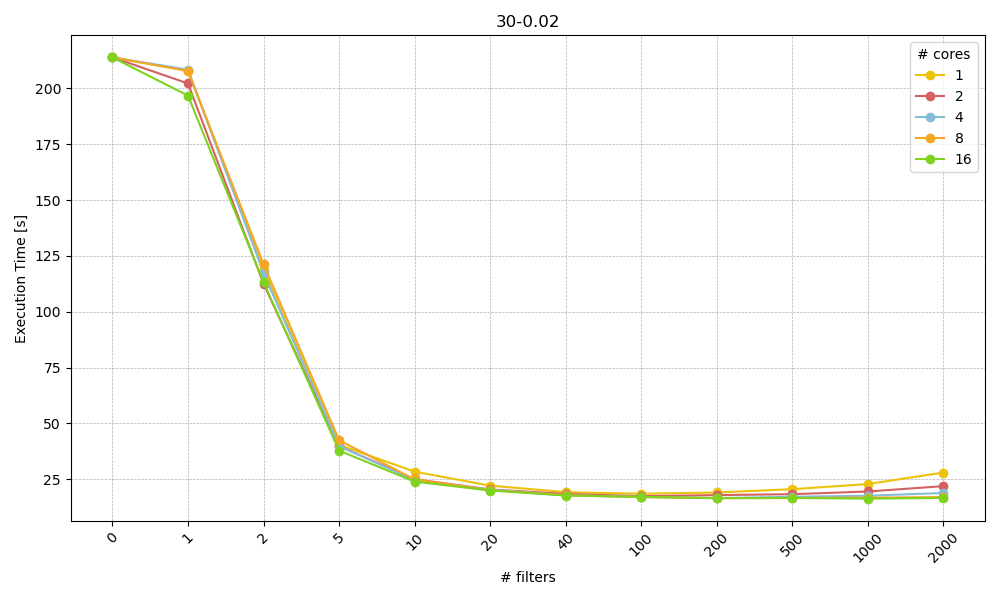
\includegraphics[scale=0.4]{images/4-Experiments/E1-NRT/120-0.02/combined/execTime-1.png}
        \caption*{}
    \end{minipage}
    \hspace{0.16\textwidth}
    \begin{minipage}{0.5\textwidth}
        \centering
        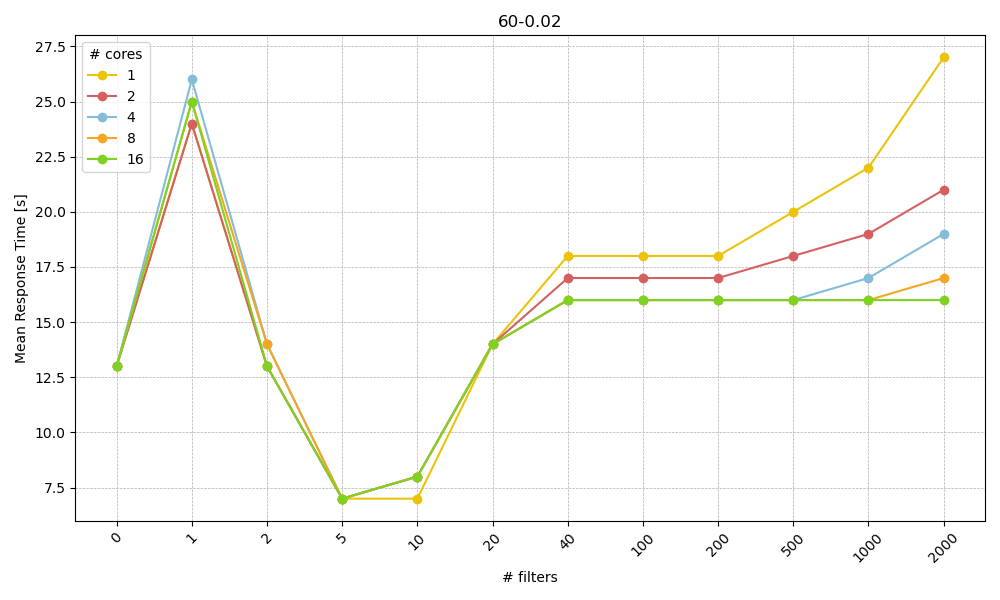
\includegraphics[scale=0.4]{images/4-Experiments/E1-NRT/120-0.02/combined/mrt-1.png}
        \caption*{}
    \end{minipage}
    
    \vspace{0.5cm} % Vertical space between rows

    \hspace*{-3cm} % Move content to the left for the second row
    \begin{minipage}{0.5\textwidth}
        \centering
        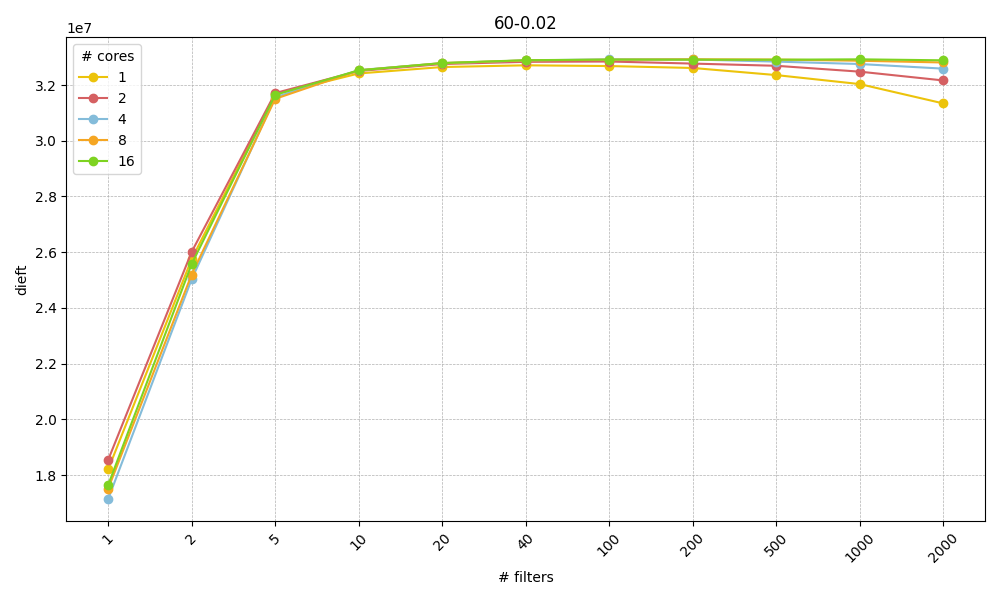
\includegraphics[scale=0.4]{images/4-Experiments/E1-NRT/120-0.02/combined/dieft-1.png}
        \caption*{}
    \end{minipage}
    \hspace{0.16\textwidth}
    \begin{minipage}{0.5\textwidth}
        \centering
        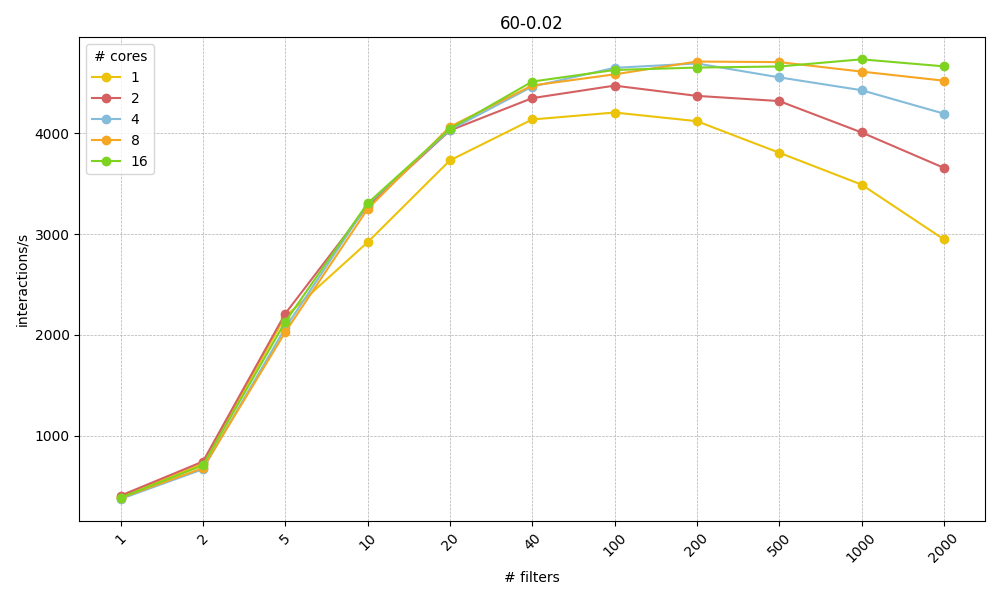
\includegraphics[scale=0.4]{images/4-Experiments/E1-NRT/120-0.02/combined/interactions-1.png}
        \caption*{}
    \end{minipage}

    \caption{Combined cores and filters variation plots for big stream: 120-0.02}
    \label{img:exps-small-120-combined}
\end{figure}

\fmc{Decidir qué poner, redactar bien las interpretaciones}
Interpretation:
\begin{itemize}
     \item \ref{img:exps-small-responsetimetraces-16c} For the smallest stream size 
     the response time of 1f (sequential) is always higher than when using more filters. However for larger stream sizes this is not the case, since from a certain point the response time tends to be higher, showing an accumulation... overhead?
     \item Conclusions: less filters maintain constant the RT (especially better for large stream sizes / where we have longer periods of high loaded scenarios). More filters however tend to get increased their response time, accumulating. In the middle, 5, 10 and 20 filters tend to be the best tradeoff between low and constant response time and low execution time / time needed to process all the input stream.
     \item The continuous behavior is better while increasing the number of filters for all the number of cores variations in terms of the \texttt{dief@t} metric, this can be seen in the \texttt{dief@t} plot in the Figure \ref{img:exps-small-120-combined}. It can also be seen in the traces plot in Figure \ref{img:exps-small-traces-16c} which shows the result traces in the case of the variations run with 16c. Note the slight degradation of the \texttt{dief@t} in the variations with the highest number of filters (from 100 and on, but specially on the cases with 1000 and 2000 filters), in the variations run with low number of cores: Figure \ref{img:exps-small-120-combined}.
     \item However measuring the behavior in terms of the execution time (total needed time to process the full stream input) and the mean response time and response time traces, we can see that for a same core configuration (e.g. 16 cores), the total execution time (time to process all the stream input) is larger for the approaches with less filters, tending to decrease. However the behavior in terms of the response time is different: the best is observed for a number of filters in the range of 5-10 filters. From that point and on the mean response time tends to degrade when increasing the number filters, especially for bigger stream sizes. Even larger than the lowest number of filters version (close to a sequential version) in these cases. This can be due to an overhead on the number of goroutines utilized and the overhead in the communication of the pipeline that this is causing.
\end{itemize}


\paragraph{Comparison of behavior depending on the number of cores}
\begin{itemize}
    \item More cores help to improve the behavior, especially for the variants with large number of filters (expected).
\end{itemize}

\begin{figure}[H]
    \centering
    % Temporarily adjust margins for wider content
    \makebox[\textwidth][c]{%
        \begin{minipage}{0.5\textwidth}
            \centering
            \includegraphics[scale=0.6]{images/4-Experiments/E1-NRT/120-0.02/fixedfilters/5f/execTime.png}
            \caption*{}
        \end{minipage}
        \hspace{0.08\textwidth}
        \begin{minipage}{0.5\textwidth}
            \centering
            \includegraphics[scale=0.6]{images/4-Experiments/E1-NRT/120-0.02/fixedfilters/20f/execTime.png}
            \caption*{}
        \end{minipage}
    }
    
    \vspace{0.5cm} % Vertical space between rows

    \makebox[\textwidth][c]{%
        \begin{minipage}{0.5\textwidth}
            \centering
            \includegraphics[scale=0.6]{images/4-Experiments/E1-NRT/120-0.02/fixedfilters/100f/execTime.png}
            \caption*{}
        \end{minipage}
        \hspace{0.08\textwidth}
        \begin{minipage}{0.5\textwidth}
            \centering
            \includegraphics[scale=0.6]{images/4-Experiments/E1-NRT/120-0.02/fixedfilters/1000f/execTime.png}
            \caption*{}
        \end{minipage}
    }

    \caption{Execution Time Fixed filters plots for stream 120-0.02}
    \label{img:exps-read-input-variants}
\end{figure}

\begin{figure}[H]
    \centering
    % Temporarily adjust margins for wider content
    \makebox[\textwidth][c]{%
        \begin{minipage}{0.5\textwidth}
            \centering
            \includegraphics[scale=0.6]{images/4-Experiments/E1-NRT/120-0.02/fixedfilters/5f/mrt.png}
            \caption*{}
        \end{minipage}
        \hspace{0.08\textwidth}
        \begin{minipage}{0.5\textwidth}
            \centering
            \includegraphics[scale=0.6]{images/4-Experiments/E1-NRT/120-0.02/fixedfilters/20f/mrt.png}
            \caption*{}
        \end{minipage}
    }
    
    \vspace{0.5cm} % Vertical space between rows

    \makebox[\textwidth][c]{%
        \begin{minipage}{0.5\textwidth}
            \centering
            \includegraphics[scale=0.6]{images/4-Experiments/E1-NRT/120-0.02/fixedfilters/100f/mrt.png}
            \caption*{}
        \end{minipage}
        \hspace{0.08\textwidth}
        \begin{minipage}{0.5\textwidth}
            \centering
            \includegraphics[scale=0.6]{images/4-Experiments/E1-NRT/120-0.02/fixedfilters/1000f/mrt.png}
            \caption*{}
        \end{minipage}
    }

    \caption{Mean Response Time Fixed filters plots for stream 120-0.02}
    \label{img:exps-read-input-variants}
\end{figure}

\subsubsection{Medium Bank Size}
  
\textcolor{red}{For these experiments, to generate the stream of tx, we needed to simplify this process in order to be able to generate a stream in a feasible amount of time. In particular we used the simplifed version of the \texttt{txGenerator.py}: \texttt{txGenerator-simplified.py} $\rightarrow$ with a random ATM-subset instead of a closest to client ATM-subset. Also variation on the transaction distribution times.}
  


Run with:
\begin{itemize}
    \item 16GB RAM
    \item x1 run each job
\end{itemize}


\subsection*{E2: Evaluation in a Real-World Stress Scenario}

\fmc{TODO: Describir y poner resultados}
For the experiments perform The real-case scenario and the high loaded test scenario. In the first case, the interactions, although read by a file of artificial simulated interactions, are provided to the pipeline data stream in such a way that they simulate their actual arrival time to the system, with the corresponding time separation between them. In the second case, the interactions are provided just one after the other as fast as possible as they are read.\\

\fmc{TODO: Describir la configuración/entorno donde corrimos los experimentos - maquinas del cluster, con + o - RAM... poner sus características}

\end{document}